\documentclass[tikz]{standalone}

\usepackage{anyfontsize}
% 各卷共用的数学记号。课程专用记号见相应的主入口。
\RequirePackage{amsmath,amssymb,bm,upgreek}

% 数集与函数空间
\newcommand*{\NN}{\mathbb{N}}
\newcommand*{\ZZ}{\mathbb{Z}}
\newcommand*{\QQ}{\mathbb{Q}}
\newcommand*{\RR}{\mathbb{R}}
\newcommand*{\CC}{\mathbb{C}}
\newcommand*{\FF}{\mathbb{F}}
\newcommand*{\cont}{\mathcal{C}}  % 连续函数空间，\cont^k 表示 k 次连续可微
\newcommand*{\poly}{\mathcal{P}}  % \poly_n 中多项式的次数至多为 n

% 微分与常数。文本中的无点 i 和字母下加点另有明确的命令。
\NewCommandCopy{\dotlessi}{\i}
\NewCommandCopy{\dotbelow}{\d}
\renewcommand*{\i}{\mathrm{i}}
\newcommand*{\nd}{\mathrm{d}}
\renewcommand*{\d}{\mathop{}\!\mathrm{d}}
\newcommand*{\e}{\mathop{}\!\mathrm{e}}
\newcommand*{\const}{\mathrm{const}}
\newcommand*{\vd}{\mathop{}\!\delta}  % 变分、依赖过程的热量或功的微元
\newcommand*{\p}{\partial}
\newcommand{\dd}[2][]{\frac{\d^{#1}}{\nd{#2}^{#1}}}
\newcommand{\dv}[3][]{\frac{\d^{#1}#2}{\nd{#3}^{#1}}}
\newcommand{\pp}[2][]{\frac{\p^{#1}}{\p{#2}^{#1}}}
\newcommand{\pv}[3][]{\frac{\p^{#1}#2}{\p{#3}^{#1}}}
\newcommand{\pw}[3]{\frac{\p^2{#1}}{\p{#2}\p{#3}}}

% 函数与算符
\let\Re\relax
\let\Im\relax
\DeclareMathOperator{\Re}{Re}
\DeclareMathOperator{\Im}{Im}
\DeclareMathOperator{\sech}{sech}
\DeclareMathOperator{\csch}{csch}
\DeclareMathOperator{\sinc}{sinc}
\DeclareMathOperator{\sgn}{sgn}
\DeclareMathOperator{\id}{id}
\DeclareMathOperator{\PV}{PV}
\DeclareMathOperator{\FT}{\mathcal{F}}
\DeclareMathOperator{\Beta}{B}
\DeclareMathOperator*{\argmin}{arg\,min}
\DeclareMathOperator*{\argmax}{arg\,max}
\newcommand*{\bigo}{\mathcal{O}}
\newcommand*{\intR}{\int_{-\infty}^\infty}
\newcommand*{\intRplus}{\int_0^\infty}

% 矢量、线性代数与场算符
\newcommand*{\hatbm}[1]{\hat{\bm{#1}}} % 带帽的粗体符号，含义随卷定义
\newcommand*{\dotbm}[1]{\dot{\bm{#1}}}
\newcommand*{\uvec}[1]{\mathop{}\!\hatbm{#1}}  % 系数后自动留薄空；单独取负写 -{\uvec n}
\newcommand*{\grad}{\nabla}
\renewcommand*{\div}{\nabla\cdot}
\newcommand*{\curl}{\nabla\times}
\newcommand*{\laplacian}{\nabla^2}
\DeclareMathOperator{\rank}{rank}
\DeclareMathOperator{\diag}{diag}
\DeclareMathOperator{\tr}{tr}
\DeclareMathOperator{\Span}{span}
\DeclareMathOperator{\nullsp}{N}
\DeclareMathOperator{\colsp}{C}
\newcommand*{\transp}{^\top}
\newcommand*{\conj}{^\ast}
\newcommand*{\adjoint}{^\dagger}
\newcommand*{\inv}{^{-1}}

% 概率、统计与物理量
\renewcommand*{\P}{\operatorname{P}}  % 段落符号 ¶ 可用 \textparagraph
\DeclareMathOperator{\E}{E}
\DeclareMathOperator{\Var}{Var}
\DeclareMathOperator{\BinDist}{Bin}
\DeclareMathOperator{\NormalDist}{N}
\newcommand*{\avg}[1]{\overline{#1}}
\newcommand*{\NA}{N_{\mathrm{A}}}
\newcommand*{\kB}{k_{\mathrm{B}}}
\newcommand*{\muB}{\mu_{\mathrm{B}}}
\newcommand*{\Ek}{E_{\mathrm{k}}}
\newcommand*{\FWHM}{\mathrm{FWHM}}
\newcommand*{\electron}{\mathrm{e}}       % 粒子标签，如 m_\electron
\newcommand*{\proton}{\mathrm{p}}
\newcommand*{\nucleus}{\mathrm{N}}
\newcommand*{\excitedstate}{\mathrm{e}}
\newcommand*{\groundstate}{\mathrm{g}}
\newcommand*{\CM}{\mathrm{CM}}
\newcommand*{\transv}{\mathrm t}  % 横向分量或模式的标签
\newcommand*{\longit}{\mathrm l}  % 纵向分量或模式的标签
\newcommand*{\electric}{\mathrm e}
\newcommand*{\magnetic}{\mathrm m}
\newcommand*{\incident}{\mathrm i}
\newcommand*{\initial}{\mathrm i}
\newcommand*{\final}{\mathrm f}
\newcommand*{\hi}{\mathrm{hi}}
\newcommand*{\lo}{\mathrm{lo}}
\newcommand*{\eff}{\mathrm{eff}}
\newcommand*{\tot}{\mathrm{tot}}

% 括号与 Dirac 记号。显式声明让公式预览也能读到每个尺寸的命令。
\newcommand{\abs}[1]{\lvert#1\rvert}
\newcommand{\bigabs}[1]{\bigl\lvert#1\bigr\rvert}
\newcommand{\Bigabs}[1]{\Bigl\lvert#1\Bigr\rvert}
\newcommand{\biggabs}[1]{\biggl\lvert#1\biggr\rvert}
\newcommand{\Biggabs}[1]{\Biggl\lvert#1\Biggr\rvert}

\newcommand{\norm}[1]{\lVert#1\rVert}
\newcommand{\bignorm}[1]{\bigl\lVert#1\bigr\rVert}
\newcommand{\Bignorm}[1]{\Bigl\lVert#1\Bigr\rVert}
\newcommand{\biggnorm}[1]{\biggl\lVert#1\biggr\rVert}
\newcommand{\Biggnorm}[1]{\Biggl\lVert#1\Biggr\rVert}

\newcommand{\eval}[1]{{#1}\rvert}
\newcommand{\bigeval}[1]{{#1}\bigr\rvert}
\newcommand{\Bigeval}[1]{{#1}\Bigr\rvert}
\newcommand{\biggeval}[1]{{#1}\biggr\rvert}
\newcommand{\Biggeval}[1]{{#1}\Biggr\rvert}

\newcommand{\floor}[1]{\lfloor#1\rfloor}
\newcommand{\bigfloor}[1]{\bigl\lfloor#1\bigr\rfloor}
\newcommand{\Bigfloor}[1]{\Bigl\lfloor#1\Bigr\rfloor}
\newcommand{\biggfloor}[1]{\biggl\lfloor#1\biggr\rfloor}
\newcommand{\Biggfloor}[1]{\Biggl\lfloor#1\Biggr\rfloor}

\newcommand{\ceil}[1]{\lceil#1\rceil}
\newcommand{\bigceil}[1]{\bigl\lceil#1\bigr\rceil}
\newcommand{\Bigceil}[1]{\Bigl\lceil#1\Bigr\rceil}
\newcommand{\biggceil}[1]{\biggl\lceil#1\biggr\rceil}
\newcommand{\Biggceil}[1]{\Biggl\lceil#1\Biggr\rceil}

\newcommand{\ave}[1]{\langle#1\rangle}
\newcommand{\bigave}[1]{\bigl\langle#1\bigr\rangle}
\newcommand{\Bigave}[1]{\Bigl\langle#1\Bigr\rangle}
\newcommand{\biggave}[1]{\biggl\langle#1\biggr\rangle}
\newcommand{\Biggave}[1]{\Biggl\langle#1\Biggr\rangle}

\newcommand{\set}[2]{\{#1\,\vert\,#2\}}
\newcommand{\bigset}[2]{\bigl\{#1\,\big\vert\,#2\bigr\}}
\newcommand{\Bigset}[2]{\Bigl\{#1\,\Big\vert\,#2\Bigr\}}
\newcommand{\biggset}[2]{\biggl\{#1\,\bigg\vert\,#2\biggr\}}
\newcommand{\Biggset}[2]{\Biggl\{#1\,\Bigg\vert\,#2\Biggr\}}

\newcommand{\division}[2]{{#1}/{#2}}
\newcommand{\bigdivision}[2]{{#1}\big/{#2}}
\newcommand{\Bigdivision}[2]{{#1}\Big/{#2}}
\newcommand{\biggdivision}[2]{{#1}\bigg/{#2}}
\newcommand{\Biggdivision}[2]{{#1}\Bigg/{#2}}

\newcommand{\inp}[2]{\langle#1,#2\rangle}
\newcommand{\biginp}[2]{\bigl\langle#1,#2\bigr\rangle}
\newcommand{\Biginp}[2]{\Bigl\langle#1,#2\Bigr\rangle}
\newcommand{\bigginp}[2]{\biggl\langle#1,#2\biggr\rangle}
\newcommand{\Bigginp}[2]{\Biggl\langle#1,#2\Biggr\rangle}

\newcommand{\bra}[1]{\langle#1\rvert}
\newcommand{\bigbra}[1]{\bigl\langle#1\bigr\rvert}
\newcommand{\Bigbra}[1]{\Bigl\langle#1\Bigr\rvert}
\newcommand{\biggbra}[1]{\biggl\langle#1\biggr\rvert}
\newcommand{\Biggbra}[1]{\Biggl\langle#1\Biggr\rvert}

\newcommand{\ket}[1]{\lvert#1\rangle}
\newcommand{\bigket}[1]{\bigl\lvert#1\bigr\rangle}
\newcommand{\Bigket}[1]{\Bigl\lvert#1\Bigr\rangle}
\newcommand{\biggket}[1]{\biggl\lvert#1\biggr\rangle}
\newcommand{\Biggket}[1]{\Biggl\lvert#1\Biggr\rangle}

\newcommand{\braket}[2]{\langle#1\vert#2\rangle}
\newcommand{\bigbraket}[2]{\bigl\langle#1\big\vert#2\bigr\rangle}
\newcommand{\Bigbraket}[2]{\Bigl\langle#1\Big\vert#2\Bigr\rangle}
\newcommand{\biggbraket}[2]{\biggl\langle#1\bigg\vert#2\biggr\rangle}
\newcommand{\Biggbraket}[2]{\Biggl\langle#1\Bigg\vert#2\Biggr\rangle}

\newcommand{\mel}[3]{\langle#1\vert#2\vert#3\rangle}
\newcommand{\bigmel}[3]{\bigl\langle#1\big\vert#2\big\vert#3\bigr\rangle}
\newcommand{\Bigmel}[3]{\Bigl\langle#1\Big\vert#2\Big\vert#3\Bigr\rangle}
\newcommand{\biggmel}[3]{\biggl\langle#1\bigg\vert#2\bigg\vert#3\biggr\rangle}
\newcommand{\Biggmel}[3]{\Biggl\langle#1\Bigg\vert#2\Bigg\vert#3\Biggr\rangle}

\newcommand{\ketbra}[2]{\lvert#1\rangle\langle#2\rvert}
\newcommand{\bigketbra}[2]{\bigl\lvert#1\bigr\rangle\bigl\langle#2\bigr\rvert}
\newcommand{\Bigketbra}[2]{\Bigl\lvert#1\Bigr\rangle\Bigl\langle#2\Bigr\rvert}
\newcommand{\biggketbra}[2]{\biggl\lvert#1\biggr\rangle\biggl\langle#2\biggr\rvert}
\newcommand{\Biggketbra}[2]{\Biggl\lvert#1\Biggr\rangle\Biggl\langle#2\Biggr\rvert}

% 兼容旧版笔记中的内积与外积命令。
\let\brkt\braket
\let\bigbrkt\bigbraket
\let\Bigbrkt\Bigbraket
\let\biggbrkt\biggbraket
\let\Biggbrkt\Biggbraket
\let\ktbr\ketbra
\let\bigktbr\bigketbra
\let\Bigktbr\Bigketbra
\let\biggktbr\biggketbra
\let\Biggktbr\Biggketbra

\newcommand{\bigp}[1]{\bigl(#1\bigr)}
\newcommand{\Bigp}[1]{\Bigl(#1\Bigr)}
\newcommand{\biggp}[1]{\biggl(#1\biggr)}
\newcommand{\Biggp}[1]{\Biggl(#1\Biggr)}

\newcommand{\bigb}[1]{\bigl[#1\bigr]}
\newcommand{\Bigb}[1]{\Bigl[#1\Bigr]}
\newcommand{\biggb}[1]{\biggl[#1\biggr]}
\newcommand{\Biggb}[1]{\Biggl[#1\Biggr]}

\newcommand{\bigB}[1]{\bigl\{#1\bigr\}}
\newcommand{\BigB}[1]{\Bigl\{#1\Bigr\}}
\newcommand{\biggB}[1]{\biggl\{#1\biggr\}}
\newcommand{\BiggB}[1]{\Biggl\{#1\Biggr\}}

% 公式排版
% 方程组的内容是一个 aligned 块，左花括号随整组方程的高度伸展。
\newcommand{\eqnset}[1]{\left\{#1\right.}
\newcommand{\fracdisp}[2]{\frac{\displaystyle #1}{\displaystyle #2}}
\newcommand*{\vs}{\mathord{\text{–}}}
\newcommand*{\otherwise}{\text{otherwise}}
\newcommand*{\qqquad}{\qquad\quad}
\newcommand*{\qqqquad}{\qquad\qquad}

\renewcommand*{\le}{\leqslant}
\renewcommand*{\leq}{\leqslant}
\renewcommand*{\ge}{\geqslant}
\renewcommand*{\geq}{\geqslant}


\begin{document}

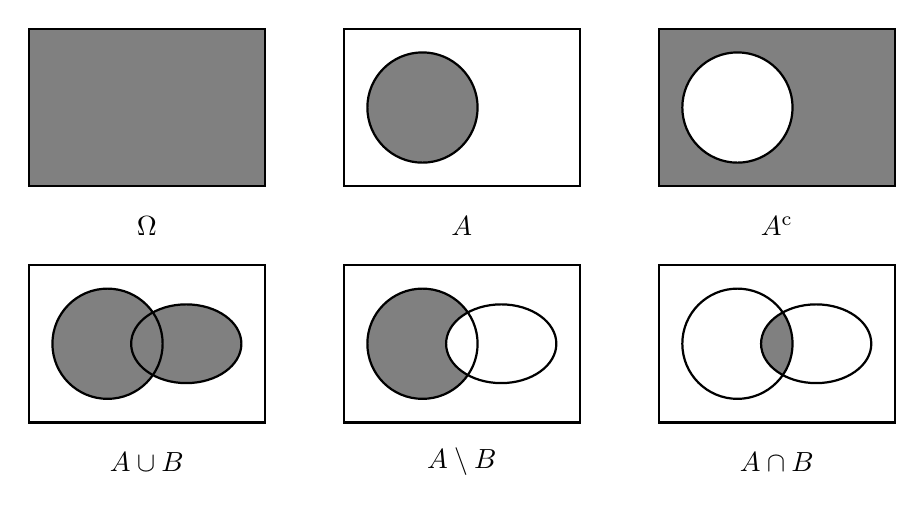
\begin{tikzpicture}
    \label{venn}
    \begin{scope}
        \draw[thick, fill=gray] (0, 0) rectangle (3, 2);
        \node at (1.5, -0.5) {$\Omega$};
    \end{scope}
    \begin{scope}[xshift=4cm]
        \draw[thick, fill=white] (0, 0) rectangle (3, 2);
        \draw[thick, fill=gray] (1, 1) circle (.7);
        \node at (1.5, -0.5) {$A$};
    \end{scope}
    \begin{scope}[xshift=8cm]
        \draw[thick, fill=gray] (0, 0) rectangle (3, 2);
        \draw[thick, fill=white] (1, 1) circle (.7);
        \node at (1.5, -0.5) {$A^{\mathrm{c}}$};
    \end{scope}
    \begin{scope}[yshift=-3cm]
        \draw[thick, fill=white] (0, 0) rectangle (3, 2);
        \fill[gray] (1, 1) circle (.7) (2, 1) ellipse (.7 and .5);
        \draw[thick] (1, 1) circle (.7);
        \draw[thick] (2, 1) ellipse (.7 and .5);
        \node at (1.5, -0.5) {$A \cup B$};
    \end{scope}
    \begin{scope}[yshift=-3cm, xshift=4cm]
        \draw[thick, fill=white] (0, 0) rectangle (3, 2);
        \fill[gray] (1, 1) circle (.7);
        \draw[thick, fill=white] (2, 1) ellipse (.7 and .5);
        \draw[thick] (1, 1) circle (.7);
        \node at (1.5, -0.5) {$A \setminus B$};
    \end{scope}
    \begin{scope}[yshift=-3cm, xshift=8cm]
        \draw[thick, fill=white] (0, 0) rectangle (3, 2);
        \begin{scope}
            \clip (1, 1) circle (.7);
            \fill[gray] (2, 1) ellipse (.7 and .5);
        \end{scope}
        \draw[thick] (1, 1) circle (.7);
        \draw[thick] (2, 1) ellipse (.7 and .5);
        \node at (1.5, -0.5) {$A \cap B$};
    \end{scope}
\end{tikzpicture}

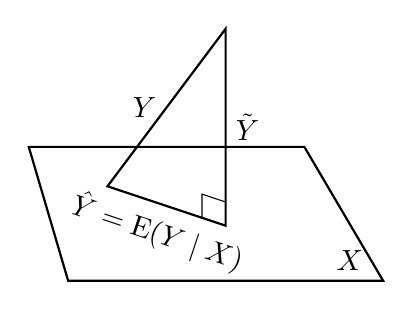
\begin{tikzpicture}[font=\fontsize{10.5bp}{12.6bp}\selectfont]
    \label{conditional-expectation}
    \draw[thick](0, 0)--(1.5, 2)node[midway, left]{$Y$}--(1.5, -.5)node[midway, right]{$\tilde Y$}--cycle node[midway, sloped, below]{$\hat Y = \E(Y \mid X)$};
    \draw(1.2, -.4)--(1.2, -.1)--(1.5, -.2);
    \draw[thick](-1, .5)--(2.5, .5)--(3.5, -1.2)node[above left]{$X~$}--(-.5, -1.2)--cycle;
\end{tikzpicture}

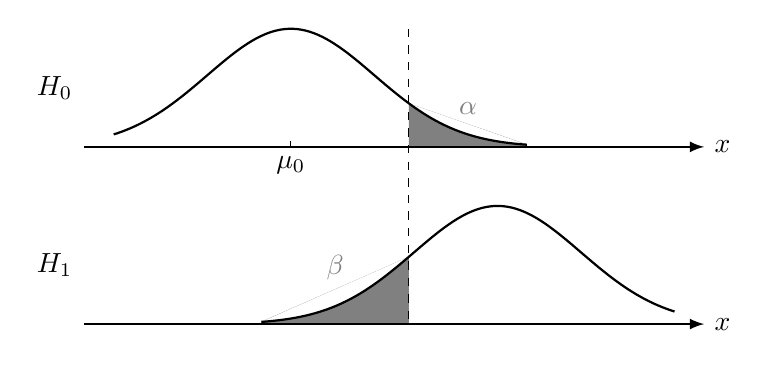
\begin{tikzpicture}[>=latex, xscale=1.5, yscale=1.5]
    \label{type-error}
    \node at(-2, .5){$H_0$};
    \node at(-2, -1){$H_1$};
    \fill[gray](1, 0)--(1, .368)--(2, .02)node[midway, above]{$\alpha$}--(2, 0);
    \fill[white, domain=1:2]plot(\x,{exp(-\x*\x)});
    \fill[gray, shift={(1.75, -1.5)}](-.75, 0)--(-.75, .57)--(-2, .02)node[midway, above]{$\beta$}--(-2, 0);
    \fill[white, domain=-2:-.75, shift={(1.75, -1.5)}]plot(\x,{exp(-\x*\x)});
    \draw[dashed](1, 1)--(1, -1.5);
    \draw[thick, -latex](-1.75, 0)--(3.5, 0)node[right]{$x$};
    \draw(0, .05)--(0, 0)node[below]{$\mu_0$};
    \draw[thick, domain=-1.5:2, samples=100]plot(\x,{exp(-\x*\x)});
    \draw[thick, -latex](-1.75, -1.5)--(3.5, -1.5)node[right]{$x$};
    \draw[thick, domain=-2:1.5, samples=100, shift={(1.75, -1.5)}]plot(\x,{exp(-\x*\x)});
\end{tikzpicture}

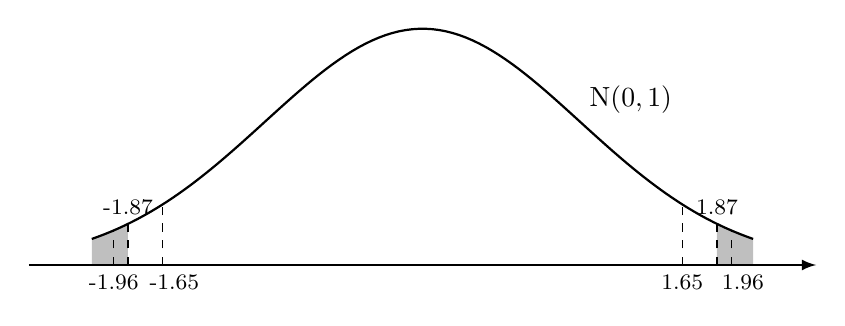
\begin{tikzpicture}[xscale=2, yscale=3]
    \label{p-value}
    \fill[gray!50](-2.1, 0)--(-2.1, 0.11)--(-1.87, 0.174)--(-1.87,0);
    \fill[gray!50](2.1, 0)--(2.1, 0.11)--(1.87, 0.174)--(1.87,0);
    \draw[thick, -latex](-2.5, 0)--(2.5, 0);
    \draw[thick, domain=-2.1:2.1, samples=100]plot(\x,{exp(-\x*\x/2)});
    \node[above right]at(1, 0.6){$\NormalDist(0,1)$};
    \draw[dashed](1.65, 0)node[below]{\footnotesize 1.65}--(1.65, 0.256);
    \draw[dashed](1.87, 0)--(1.87, 0.174)node[above]{\footnotesize 1.87};
    \draw[dashed](1.96, 0)node[below]{\footnotesize\quad 1.96}--(1.96, 0.146);
    \draw[dashed](-1.65, 0)node[below]{\footnotesize\quad -1.65}--(-1.65, 0.256);
    \draw[dashed](-1.87, 0)--(-1.87, 0.174)node[above]{\footnotesize -1.87};
    \draw[dashed](-1.96, 0)node[below]{\footnotesize -1.96}--(-1.96, 0.146);
\end{tikzpicture}

% ref: https://tikz.net/venn-diagrams/
% author: Jake
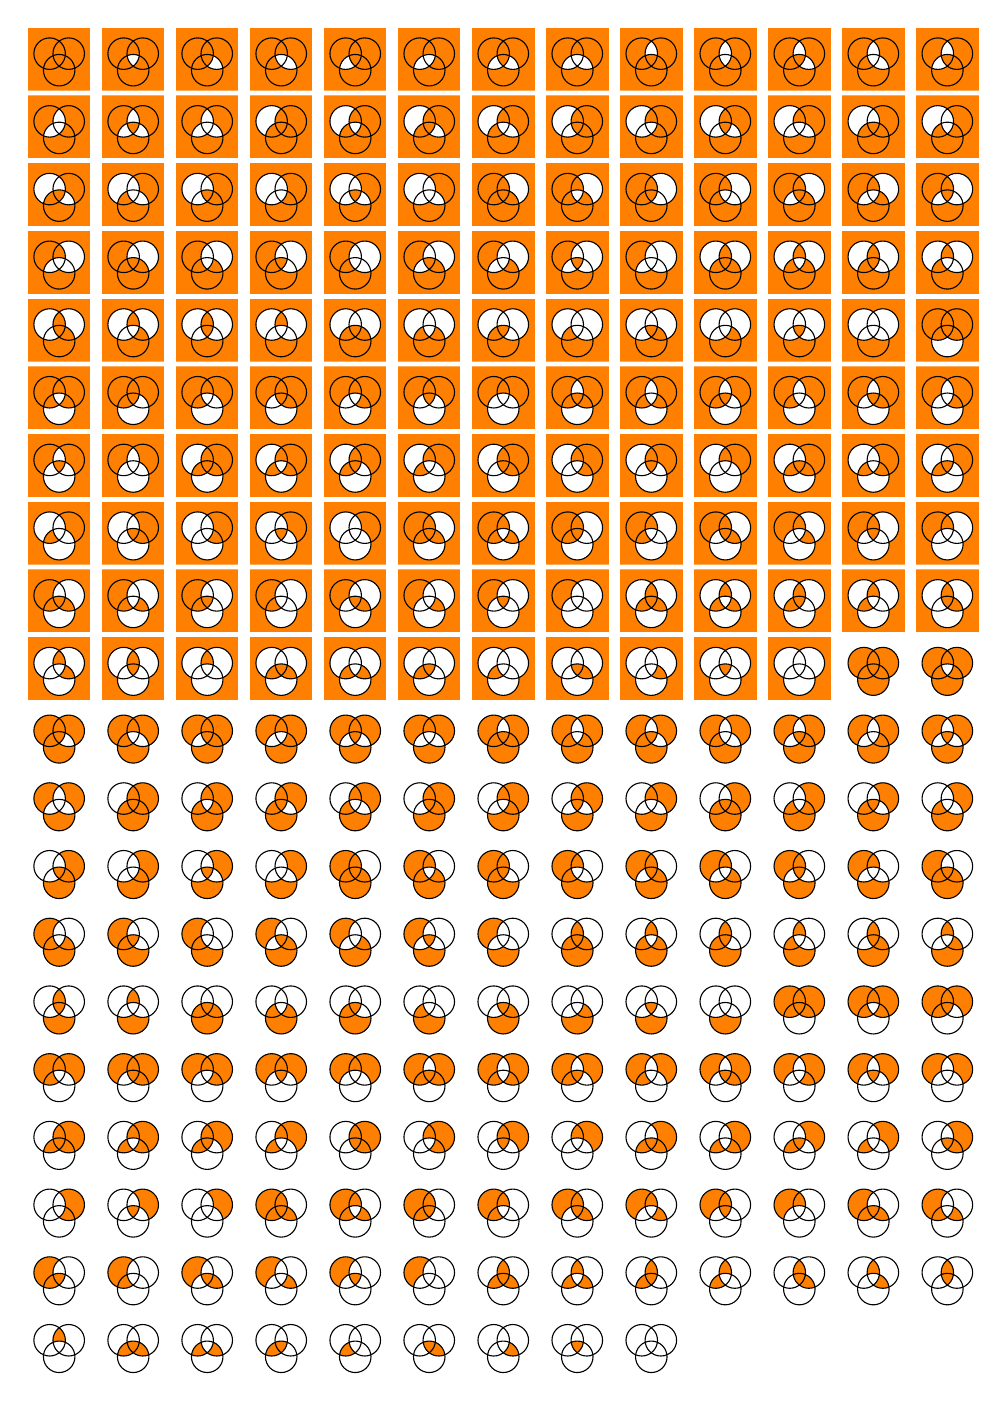
\begin{tikzpicture}[scale=0.2]
    \label{venn-three-sets}
    \tikzset{reverseclip/.style={insert path={
        (2,2) -- (2,-2) -- (-2,-2) -- (-2,2) -- cycle}}}

    \tikzset{
        venn0/.code={
            \begin{scope}
                \begin{pgfinterruptboundingbox}
                \path  [clip] (-90:0.7cm) circle [radius=1cm] [reverseclip];
                \path  [clip] (30:0.7cm) circle [radius=1cm] [reverseclip];
                \path  [clip] (-210:0.7cm) circle [radius=1cm] [reverseclip];
                \end{pgfinterruptboundingbox}
                \fill [orange] (-2,-2) rectangle (2,2);
            \end{scope}
        },
        venn1/.code={
            \begin{scope}
                \begin{pgfinterruptboundingbox}
                \path  [clip] (-90:0.7cm) circle [radius=1cm];
                \path  [clip] (30:0.7cm) circle [radius=1cm] [reverseclip];
                \path  [clip] (-210:0.7cm) circle [radius=1cm] [reverseclip];
                \end{pgfinterruptboundingbox}
                \fill [orange] (-2,-2) rectangle (2,2);
            \end{scope}
        },
        venn2/.code={
            \begin{scope}
                \begin{pgfinterruptboundingbox}
                \path  [clip] (-90:0.7cm) circle [radius=1cm] [reverseclip];
                \path  [clip] (30:0.7cm) circle [radius=1cm];
                \path  [clip] (-210:0.7cm) circle [radius=1cm] [reverseclip];
                \end{pgfinterruptboundingbox}
                \fill [orange] (-2,-2) rectangle (2,2);
            \end{scope}
        },
        venn3/.code={
            \begin{scope}
                \begin{pgfinterruptboundingbox}
                \path  [clip] (-90:0.7cm) circle [radius=1cm] [reverseclip];
                \path  [clip] (30:0.7cm) circle [radius=1cm] [reverseclip];
                \path  [clip] (-210:0.7cm) circle [radius=1cm];
                \end{pgfinterruptboundingbox}
                \fill [orange] (-2,-2) rectangle (2,2);
            \end{scope}
        },
        venn4/.code={
            \begin{scope}
                \begin{pgfinterruptboundingbox}
                \path  [clip] (-90:0.7cm) circle [radius=1cm] [reverseclip];
                \path  [clip] (30:0.7cm) circle [radius=1cm] ;
                \path  [clip] (-210:0.7cm) circle [radius=1cm] ;
                \end{pgfinterruptboundingbox}
                \fill [orange] (-2,-2) rectangle (2,2);
            \end{scope}
        },
        venn5/.code={
            \begin{scope}
                \begin{pgfinterruptboundingbox}
                \path  [clip] (-90:0.7cm) circle [radius=1cm];
                \path  [clip] (30:0.7cm) circle [radius=1cm] [reverseclip];
                \path  [clip] (-210:0.7cm) circle [radius=1cm];
                \end{pgfinterruptboundingbox}
                \fill [orange] (-2,-2) rectangle (2,2);
            \end{scope}
        },
        venn6/.code={
            \begin{scope}
                \begin{pgfinterruptboundingbox}
                \path  [clip] (-90:0.7cm) circle [radius=1cm];
                \path  [clip] (30:0.7cm) circle [radius=1cm] ;
                \path  [clip] (-210:0.7cm) circle [radius=1cm] [reverseclip];
                \end{pgfinterruptboundingbox}
                \fill [orange] (-2,-2) rectangle (2,2);
            \end{scope}
        },
        venn7/.code={
            \begin{scope}
                \begin{pgfinterruptboundingbox}
                \path  [clip] (-90:0.7cm) circle [radius=1cm];
                \path  [clip] (30:0.7cm) circle [radius=1cm] ;
                \path  [clip] (-210:0.7cm) circle [radius=1cm];
                \end{pgfinterruptboundingbox}
                \fill [orange] (-2,-2) rectangle (2,2);
            \end{scope}
        },
        vennoutlines/.code={
            \draw (-90:0.7cm) circle [radius=1cm];
            \draw (30:0.7cm) circle [radius=1cm];
            \draw (-210:0.7cm) circle [radius=1cm];
        }
    }

    % Each 8-bit mask selects one of the 256 shadings of the eight regions.
    \foreach \mask in {0,...,255} {
        \begin{scope}[shift={({4.7*mod(\mask,13)},{-4.3*floor(\mask/13)})}]
            \foreach \region in {0,...,7} {
                \pgfmathtruncatemacro{\bit}{mod(floor(\mask/2^(7-\region)),2)}
                \ifnum\bit=0 \tikzset{venn\region}\fi
            }
            \tikzset{vennoutlines}
        \end{scope}
    }
\end{tikzpicture}

\end{document}
